\documentclass[xcolor=dvipsnames, compress, serif, professionalfont, handout]{beamer}
\usepackage{graphicx, color}
\newcommand{\hlnumber}[1]{\textcolor[rgb]{0,0,0}{#1}}%
\newcommand{\hlfunctioncall}[1]{\textcolor[rgb]{.5,0,.33}{\textbf{#1}}}%
\newcommand{\hlstring}[1]{\textcolor[rgb]{.6,.6,1}{#1}}%
\newcommand{\hlkeyword}[1]{\textbf{#1}}%
\newcommand{\hlargument}[1]{\textcolor[rgb]{.69,.25,.02}{#1}}%
\newcommand{\hlcomment}[1]{\textcolor[rgb]{.18,.6,.34}{#1}}%
\newcommand{\hlroxygencomment}[1]{\textcolor[rgb]{.44,.48,.7}{#1}}%
\newcommand{\hlformalargs}[1]{\hlargument{#1}}%
\newcommand{\hleqformalargs}[1]{\hlargument{#1}}%
\newcommand{\hlassignement}[1]{\textbf{#1}}%
\newcommand{\hlpackage}[1]{\textcolor[rgb]{.59,.71,.145}{#1}}%
\newcommand{\hlslot}[1]{\textit{#1}}%
\newcommand{\hlsymbol}[1]{#1}%
\newcommand{\hlprompt}[1]{\textcolor[rgb]{.5,.5,.5}{#1}}%

\usepackage{color}%
 
\newsavebox{\hlnormalsizeboxclosebrace}%
\newsavebox{\hlnormalsizeboxopenbrace}%
\newsavebox{\hlnormalsizeboxbackslash}%
\newsavebox{\hlnormalsizeboxlessthan}%
\newsavebox{\hlnormalsizeboxgreaterthan}%
\newsavebox{\hlnormalsizeboxdollar}%
\newsavebox{\hlnormalsizeboxunderscore}%
\newsavebox{\hlnormalsizeboxand}%
\newsavebox{\hlnormalsizeboxhash}%
\newsavebox{\hlnormalsizeboxat}%
\newsavebox{\hlnormalsizeboxpercent}% 
\newsavebox{\hlnormalsizeboxhat}%
\newsavebox{\hlnormalsizeboxsinglequote}%
\newsavebox{\hlnormalsizeboxbacktick}%

\setbox\hlnormalsizeboxopenbrace=\hbox{\begin{normalsize}\verb.{.\end{normalsize}}%
\setbox\hlnormalsizeboxclosebrace=\hbox{\begin{normalsize}\verb.}.\end{normalsize}}%
\setbox\hlnormalsizeboxlessthan=\hbox{\begin{normalsize}\verb.<.\end{normalsize}}%
\setbox\hlnormalsizeboxdollar=\hbox{\begin{normalsize}\verb.$.\end{normalsize}}%
\setbox\hlnormalsizeboxunderscore=\hbox{\begin{normalsize}\verb._.\end{normalsize}}%
\setbox\hlnormalsizeboxand=\hbox{\begin{normalsize}\verb.&.\end{normalsize}}%
\setbox\hlnormalsizeboxhash=\hbox{\begin{normalsize}\verb.#.\end{normalsize}}%
\setbox\hlnormalsizeboxat=\hbox{\begin{normalsize}\verb.@.\end{normalsize}}%
\setbox\hlnormalsizeboxbackslash=\hbox{\begin{normalsize}\verb.\.\end{normalsize}}%
\setbox\hlnormalsizeboxgreaterthan=\hbox{\begin{normalsize}\verb.>.\end{normalsize}}%
\setbox\hlnormalsizeboxpercent=\hbox{\begin{normalsize}\verb.%.\end{normalsize}}%
\setbox\hlnormalsizeboxhat=\hbox{\begin{normalsize}\verb.^.\end{normalsize}}%
\setbox\hlnormalsizeboxsinglequote=\hbox{\begin{normalsize}\verb.'.\end{normalsize}}%
\setbox\hlnormalsizeboxbacktick=\hbox{\begin{normalsize}\verb.`.\end{normalsize}}%
\setbox\hlnormalsizeboxhat=\hbox{\begin{normalsize}\verb.^.\end{normalsize}}%



\newsavebox{\hltinyboxclosebrace}%
\newsavebox{\hltinyboxopenbrace}%
\newsavebox{\hltinyboxbackslash}%
\newsavebox{\hltinyboxlessthan}%
\newsavebox{\hltinyboxgreaterthan}%
\newsavebox{\hltinyboxdollar}%
\newsavebox{\hltinyboxunderscore}%
\newsavebox{\hltinyboxand}%
\newsavebox{\hltinyboxhash}%
\newsavebox{\hltinyboxat}%
\newsavebox{\hltinyboxpercent}% 
\newsavebox{\hltinyboxhat}%
\newsavebox{\hltinyboxsinglequote}%
\newsavebox{\hltinyboxbacktick}%

\setbox\hltinyboxopenbrace=\hbox{\begin{tiny}\verb.{.\end{tiny}}%
\setbox\hltinyboxclosebrace=\hbox{\begin{tiny}\verb.}.\end{tiny}}%
\setbox\hltinyboxlessthan=\hbox{\begin{tiny}\verb.<.\end{tiny}}%
\setbox\hltinyboxdollar=\hbox{\begin{tiny}\verb.$.\end{tiny}}%
\setbox\hltinyboxunderscore=\hbox{\begin{tiny}\verb._.\end{tiny}}%
\setbox\hltinyboxand=\hbox{\begin{tiny}\verb.&.\end{tiny}}%
\setbox\hltinyboxhash=\hbox{\begin{tiny}\verb.#.\end{tiny}}%
\setbox\hltinyboxat=\hbox{\begin{tiny}\verb.@.\end{tiny}}%
\setbox\hltinyboxbackslash=\hbox{\begin{tiny}\verb.\.\end{tiny}}%
\setbox\hltinyboxgreaterthan=\hbox{\begin{tiny}\verb.>.\end{tiny}}%
\setbox\hltinyboxpercent=\hbox{\begin{tiny}\verb.%.\end{tiny}}%
\setbox\hltinyboxhat=\hbox{\begin{tiny}\verb.^.\end{tiny}}%
\setbox\hltinyboxsinglequote=\hbox{\begin{tiny}\verb.'.\end{tiny}}%
\setbox\hltinyboxbacktick=\hbox{\begin{tiny}\verb.`.\end{tiny}}%
\setbox\hltinyboxhat=\hbox{\begin{tiny}\verb.^.\end{tiny}}%



\newsavebox{\hlscriptsizeboxclosebrace}%
\newsavebox{\hlscriptsizeboxopenbrace}%
\newsavebox{\hlscriptsizeboxbackslash}%
\newsavebox{\hlscriptsizeboxlessthan}%
\newsavebox{\hlscriptsizeboxgreaterthan}%
\newsavebox{\hlscriptsizeboxdollar}%
\newsavebox{\hlscriptsizeboxunderscore}%
\newsavebox{\hlscriptsizeboxand}%
\newsavebox{\hlscriptsizeboxhash}%
\newsavebox{\hlscriptsizeboxat}%
\newsavebox{\hlscriptsizeboxpercent}% 
\newsavebox{\hlscriptsizeboxhat}%
\newsavebox{\hlscriptsizeboxsinglequote}%
\newsavebox{\hlscriptsizeboxbacktick}%

\setbox\hlscriptsizeboxopenbrace=\hbox{\begin{scriptsize}\verb.{.\end{scriptsize}}%
\setbox\hlscriptsizeboxclosebrace=\hbox{\begin{scriptsize}\verb.}.\end{scriptsize}}%
\setbox\hlscriptsizeboxlessthan=\hbox{\begin{scriptsize}\verb.<.\end{scriptsize}}%
\setbox\hlscriptsizeboxdollar=\hbox{\begin{scriptsize}\verb.$.\end{scriptsize}}%
\setbox\hlscriptsizeboxunderscore=\hbox{\begin{scriptsize}\verb._.\end{scriptsize}}%
\setbox\hlscriptsizeboxand=\hbox{\begin{scriptsize}\verb.&.\end{scriptsize}}%
\setbox\hlscriptsizeboxhash=\hbox{\begin{scriptsize}\verb.#.\end{scriptsize}}%
\setbox\hlscriptsizeboxat=\hbox{\begin{scriptsize}\verb.@.\end{scriptsize}}%
\setbox\hlscriptsizeboxbackslash=\hbox{\begin{scriptsize}\verb.\.\end{scriptsize}}%
\setbox\hlscriptsizeboxgreaterthan=\hbox{\begin{scriptsize}\verb.>.\end{scriptsize}}%
\setbox\hlscriptsizeboxpercent=\hbox{\begin{scriptsize}\verb.%.\end{scriptsize}}%
\setbox\hlscriptsizeboxhat=\hbox{\begin{scriptsize}\verb.^.\end{scriptsize}}%
\setbox\hlscriptsizeboxsinglequote=\hbox{\begin{scriptsize}\verb.'.\end{scriptsize}}%
\setbox\hlscriptsizeboxbacktick=\hbox{\begin{scriptsize}\verb.`.\end{scriptsize}}%
\setbox\hlscriptsizeboxhat=\hbox{\begin{scriptsize}\verb.^.\end{scriptsize}}%



\newsavebox{\hlfootnotesizeboxclosebrace}%
\newsavebox{\hlfootnotesizeboxopenbrace}%
\newsavebox{\hlfootnotesizeboxbackslash}%
\newsavebox{\hlfootnotesizeboxlessthan}%
\newsavebox{\hlfootnotesizeboxgreaterthan}%
\newsavebox{\hlfootnotesizeboxdollar}%
\newsavebox{\hlfootnotesizeboxunderscore}%
\newsavebox{\hlfootnotesizeboxand}%
\newsavebox{\hlfootnotesizeboxhash}%
\newsavebox{\hlfootnotesizeboxat}%
\newsavebox{\hlfootnotesizeboxpercent}% 
\newsavebox{\hlfootnotesizeboxhat}%
\newsavebox{\hlfootnotesizeboxsinglequote}%
\newsavebox{\hlfootnotesizeboxbacktick}%

\setbox\hlfootnotesizeboxopenbrace=\hbox{\begin{footnotesize}\verb.{.\end{footnotesize}}%
\setbox\hlfootnotesizeboxclosebrace=\hbox{\begin{footnotesize}\verb.}.\end{footnotesize}}%
\setbox\hlfootnotesizeboxlessthan=\hbox{\begin{footnotesize}\verb.<.\end{footnotesize}}%
\setbox\hlfootnotesizeboxdollar=\hbox{\begin{footnotesize}\verb.$.\end{footnotesize}}%
\setbox\hlfootnotesizeboxunderscore=\hbox{\begin{footnotesize}\verb._.\end{footnotesize}}%
\setbox\hlfootnotesizeboxand=\hbox{\begin{footnotesize}\verb.&.\end{footnotesize}}%
\setbox\hlfootnotesizeboxhash=\hbox{\begin{footnotesize}\verb.#.\end{footnotesize}}%
\setbox\hlfootnotesizeboxat=\hbox{\begin{footnotesize}\verb.@.\end{footnotesize}}%
\setbox\hlfootnotesizeboxbackslash=\hbox{\begin{footnotesize}\verb.\.\end{footnotesize}}%
\setbox\hlfootnotesizeboxgreaterthan=\hbox{\begin{footnotesize}\verb.>.\end{footnotesize}}%
\setbox\hlfootnotesizeboxpercent=\hbox{\begin{footnotesize}\verb.%.\end{footnotesize}}%
\setbox\hlfootnotesizeboxhat=\hbox{\begin{footnotesize}\verb.^.\end{footnotesize}}%
\setbox\hlfootnotesizeboxsinglequote=\hbox{\begin{footnotesize}\verb.'.\end{footnotesize}}%
\setbox\hlfootnotesizeboxbacktick=\hbox{\begin{footnotesize}\verb.`.\end{footnotesize}}%
\setbox\hlfootnotesizeboxhat=\hbox{\begin{footnotesize}\verb.^.\end{footnotesize}}%



\newsavebox{\hlsmallboxclosebrace}%
\newsavebox{\hlsmallboxopenbrace}%
\newsavebox{\hlsmallboxbackslash}%
\newsavebox{\hlsmallboxlessthan}%
\newsavebox{\hlsmallboxgreaterthan}%
\newsavebox{\hlsmallboxdollar}%
\newsavebox{\hlsmallboxunderscore}%
\newsavebox{\hlsmallboxand}%
\newsavebox{\hlsmallboxhash}%
\newsavebox{\hlsmallboxat}%
\newsavebox{\hlsmallboxpercent}% 
\newsavebox{\hlsmallboxhat}%
\newsavebox{\hlsmallboxsinglequote}%
\newsavebox{\hlsmallboxbacktick}%

\setbox\hlsmallboxopenbrace=\hbox{\begin{small}\verb.{.\end{small}}%
\setbox\hlsmallboxclosebrace=\hbox{\begin{small}\verb.}.\end{small}}%
\setbox\hlsmallboxlessthan=\hbox{\begin{small}\verb.<.\end{small}}%
\setbox\hlsmallboxdollar=\hbox{\begin{small}\verb.$.\end{small}}%
\setbox\hlsmallboxunderscore=\hbox{\begin{small}\verb._.\end{small}}%
\setbox\hlsmallboxand=\hbox{\begin{small}\verb.&.\end{small}}%
\setbox\hlsmallboxhash=\hbox{\begin{small}\verb.#.\end{small}}%
\setbox\hlsmallboxat=\hbox{\begin{small}\verb.@.\end{small}}%
\setbox\hlsmallboxbackslash=\hbox{\begin{small}\verb.\.\end{small}}%
\setbox\hlsmallboxgreaterthan=\hbox{\begin{small}\verb.>.\end{small}}%
\setbox\hlsmallboxpercent=\hbox{\begin{small}\verb.%.\end{small}}%
\setbox\hlsmallboxhat=\hbox{\begin{small}\verb.^.\end{small}}%
\setbox\hlsmallboxsinglequote=\hbox{\begin{small}\verb.'.\end{small}}%
\setbox\hlsmallboxbacktick=\hbox{\begin{small}\verb.`.\end{small}}%
\setbox\hlsmallboxhat=\hbox{\begin{small}\verb.^.\end{small}}%



\newsavebox{\hllargeboxclosebrace}%
\newsavebox{\hllargeboxopenbrace}%
\newsavebox{\hllargeboxbackslash}%
\newsavebox{\hllargeboxlessthan}%
\newsavebox{\hllargeboxgreaterthan}%
\newsavebox{\hllargeboxdollar}%
\newsavebox{\hllargeboxunderscore}%
\newsavebox{\hllargeboxand}%
\newsavebox{\hllargeboxhash}%
\newsavebox{\hllargeboxat}%
\newsavebox{\hllargeboxpercent}% 
\newsavebox{\hllargeboxhat}%
\newsavebox{\hllargeboxsinglequote}%
\newsavebox{\hllargeboxbacktick}%

\setbox\hllargeboxopenbrace=\hbox{\begin{large}\verb.{.\end{large}}%
\setbox\hllargeboxclosebrace=\hbox{\begin{large}\verb.}.\end{large}}%
\setbox\hllargeboxlessthan=\hbox{\begin{large}\verb.<.\end{large}}%
\setbox\hllargeboxdollar=\hbox{\begin{large}\verb.$.\end{large}}%
\setbox\hllargeboxunderscore=\hbox{\begin{large}\verb._.\end{large}}%
\setbox\hllargeboxand=\hbox{\begin{large}\verb.&.\end{large}}%
\setbox\hllargeboxhash=\hbox{\begin{large}\verb.#.\end{large}}%
\setbox\hllargeboxat=\hbox{\begin{large}\verb.@.\end{large}}%
\setbox\hllargeboxbackslash=\hbox{\begin{large}\verb.\.\end{large}}%
\setbox\hllargeboxgreaterthan=\hbox{\begin{large}\verb.>.\end{large}}%
\setbox\hllargeboxpercent=\hbox{\begin{large}\verb.%.\end{large}}%
\setbox\hllargeboxhat=\hbox{\begin{large}\verb.^.\end{large}}%
\setbox\hllargeboxsinglequote=\hbox{\begin{large}\verb.'.\end{large}}%
\setbox\hllargeboxbacktick=\hbox{\begin{large}\verb.`.\end{large}}%
\setbox\hllargeboxhat=\hbox{\begin{large}\verb.^.\end{large}}%



\newsavebox{\hlLargeboxclosebrace}%
\newsavebox{\hlLargeboxopenbrace}%
\newsavebox{\hlLargeboxbackslash}%
\newsavebox{\hlLargeboxlessthan}%
\newsavebox{\hlLargeboxgreaterthan}%
\newsavebox{\hlLargeboxdollar}%
\newsavebox{\hlLargeboxunderscore}%
\newsavebox{\hlLargeboxand}%
\newsavebox{\hlLargeboxhash}%
\newsavebox{\hlLargeboxat}%
\newsavebox{\hlLargeboxpercent}% 
\newsavebox{\hlLargeboxhat}%
\newsavebox{\hlLargeboxsinglequote}%
\newsavebox{\hlLargeboxbacktick}%

\setbox\hlLargeboxopenbrace=\hbox{\begin{Large}\verb.{.\end{Large}}%
\setbox\hlLargeboxclosebrace=\hbox{\begin{Large}\verb.}.\end{Large}}%
\setbox\hlLargeboxlessthan=\hbox{\begin{Large}\verb.<.\end{Large}}%
\setbox\hlLargeboxdollar=\hbox{\begin{Large}\verb.$.\end{Large}}%
\setbox\hlLargeboxunderscore=\hbox{\begin{Large}\verb._.\end{Large}}%
\setbox\hlLargeboxand=\hbox{\begin{Large}\verb.&.\end{Large}}%
\setbox\hlLargeboxhash=\hbox{\begin{Large}\verb.#.\end{Large}}%
\setbox\hlLargeboxat=\hbox{\begin{Large}\verb.@.\end{Large}}%
\setbox\hlLargeboxbackslash=\hbox{\begin{Large}\verb.\.\end{Large}}%
\setbox\hlLargeboxgreaterthan=\hbox{\begin{Large}\verb.>.\end{Large}}%
\setbox\hlLargeboxpercent=\hbox{\begin{Large}\verb.%.\end{Large}}%
\setbox\hlLargeboxhat=\hbox{\begin{Large}\verb.^.\end{Large}}%
\setbox\hlLargeboxsinglequote=\hbox{\begin{Large}\verb.'.\end{Large}}%
\setbox\hlLargeboxbacktick=\hbox{\begin{Large}\verb.`.\end{Large}}%
\setbox\hlLargeboxhat=\hbox{\begin{Large}\verb.^.\end{Large}}%



\newsavebox{\hlLARGEboxclosebrace}%
\newsavebox{\hlLARGEboxopenbrace}%
\newsavebox{\hlLARGEboxbackslash}%
\newsavebox{\hlLARGEboxlessthan}%
\newsavebox{\hlLARGEboxgreaterthan}%
\newsavebox{\hlLARGEboxdollar}%
\newsavebox{\hlLARGEboxunderscore}%
\newsavebox{\hlLARGEboxand}%
\newsavebox{\hlLARGEboxhash}%
\newsavebox{\hlLARGEboxat}%
\newsavebox{\hlLARGEboxpercent}% 
\newsavebox{\hlLARGEboxhat}%
\newsavebox{\hlLARGEboxsinglequote}%
\newsavebox{\hlLARGEboxbacktick}%

\setbox\hlLARGEboxopenbrace=\hbox{\begin{LARGE}\verb.{.\end{LARGE}}%
\setbox\hlLARGEboxclosebrace=\hbox{\begin{LARGE}\verb.}.\end{LARGE}}%
\setbox\hlLARGEboxlessthan=\hbox{\begin{LARGE}\verb.<.\end{LARGE}}%
\setbox\hlLARGEboxdollar=\hbox{\begin{LARGE}\verb.$.\end{LARGE}}%
\setbox\hlLARGEboxunderscore=\hbox{\begin{LARGE}\verb._.\end{LARGE}}%
\setbox\hlLARGEboxand=\hbox{\begin{LARGE}\verb.&.\end{LARGE}}%
\setbox\hlLARGEboxhash=\hbox{\begin{LARGE}\verb.#.\end{LARGE}}%
\setbox\hlLARGEboxat=\hbox{\begin{LARGE}\verb.@.\end{LARGE}}%
\setbox\hlLARGEboxbackslash=\hbox{\begin{LARGE}\verb.\.\end{LARGE}}%
\setbox\hlLARGEboxgreaterthan=\hbox{\begin{LARGE}\verb.>.\end{LARGE}}%
\setbox\hlLARGEboxpercent=\hbox{\begin{LARGE}\verb.%.\end{LARGE}}%
\setbox\hlLARGEboxhat=\hbox{\begin{LARGE}\verb.^.\end{LARGE}}%
\setbox\hlLARGEboxsinglequote=\hbox{\begin{LARGE}\verb.'.\end{LARGE}}%
\setbox\hlLARGEboxbacktick=\hbox{\begin{LARGE}\verb.`.\end{LARGE}}%
\setbox\hlLARGEboxhat=\hbox{\begin{LARGE}\verb.^.\end{LARGE}}%



\newsavebox{\hlhugeboxclosebrace}%
\newsavebox{\hlhugeboxopenbrace}%
\newsavebox{\hlhugeboxbackslash}%
\newsavebox{\hlhugeboxlessthan}%
\newsavebox{\hlhugeboxgreaterthan}%
\newsavebox{\hlhugeboxdollar}%
\newsavebox{\hlhugeboxunderscore}%
\newsavebox{\hlhugeboxand}%
\newsavebox{\hlhugeboxhash}%
\newsavebox{\hlhugeboxat}%
\newsavebox{\hlhugeboxpercent}% 
\newsavebox{\hlhugeboxhat}%
\newsavebox{\hlhugeboxsinglequote}%
\newsavebox{\hlhugeboxbacktick}%

\setbox\hlhugeboxopenbrace=\hbox{\begin{huge}\verb.{.\end{huge}}%
\setbox\hlhugeboxclosebrace=\hbox{\begin{huge}\verb.}.\end{huge}}%
\setbox\hlhugeboxlessthan=\hbox{\begin{huge}\verb.<.\end{huge}}%
\setbox\hlhugeboxdollar=\hbox{\begin{huge}\verb.$.\end{huge}}%
\setbox\hlhugeboxunderscore=\hbox{\begin{huge}\verb._.\end{huge}}%
\setbox\hlhugeboxand=\hbox{\begin{huge}\verb.&.\end{huge}}%
\setbox\hlhugeboxhash=\hbox{\begin{huge}\verb.#.\end{huge}}%
\setbox\hlhugeboxat=\hbox{\begin{huge}\verb.@.\end{huge}}%
\setbox\hlhugeboxbackslash=\hbox{\begin{huge}\verb.\.\end{huge}}%
\setbox\hlhugeboxgreaterthan=\hbox{\begin{huge}\verb.>.\end{huge}}%
\setbox\hlhugeboxpercent=\hbox{\begin{huge}\verb.%.\end{huge}}%
\setbox\hlhugeboxhat=\hbox{\begin{huge}\verb.^.\end{huge}}%
\setbox\hlhugeboxsinglequote=\hbox{\begin{huge}\verb.'.\end{huge}}%
\setbox\hlhugeboxbacktick=\hbox{\begin{huge}\verb.`.\end{huge}}%
\setbox\hlhugeboxhat=\hbox{\begin{huge}\verb.^.\end{huge}}%



\newsavebox{\hlHugeboxclosebrace}%
\newsavebox{\hlHugeboxopenbrace}%
\newsavebox{\hlHugeboxbackslash}%
\newsavebox{\hlHugeboxlessthan}%
\newsavebox{\hlHugeboxgreaterthan}%
\newsavebox{\hlHugeboxdollar}%
\newsavebox{\hlHugeboxunderscore}%
\newsavebox{\hlHugeboxand}%
\newsavebox{\hlHugeboxhash}%
\newsavebox{\hlHugeboxat}%
\newsavebox{\hlHugeboxpercent}% 
\newsavebox{\hlHugeboxhat}%
\newsavebox{\hlHugeboxsinglequote}%
\newsavebox{\hlHugeboxbacktick}%

\setbox\hlHugeboxopenbrace=\hbox{\begin{Huge}\verb.{.\end{Huge}}%
\setbox\hlHugeboxclosebrace=\hbox{\begin{Huge}\verb.}.\end{Huge}}%
\setbox\hlHugeboxlessthan=\hbox{\begin{Huge}\verb.<.\end{Huge}}%
\setbox\hlHugeboxdollar=\hbox{\begin{Huge}\verb.$.\end{Huge}}%
\setbox\hlHugeboxunderscore=\hbox{\begin{Huge}\verb._.\end{Huge}}%
\setbox\hlHugeboxand=\hbox{\begin{Huge}\verb.&.\end{Huge}}%
\setbox\hlHugeboxhash=\hbox{\begin{Huge}\verb.#.\end{Huge}}%
\setbox\hlHugeboxat=\hbox{\begin{Huge}\verb.@.\end{Huge}}%
\setbox\hlHugeboxbackslash=\hbox{\begin{Huge}\verb.\.\end{Huge}}%
\setbox\hlHugeboxgreaterthan=\hbox{\begin{Huge}\verb.>.\end{Huge}}%
\setbox\hlHugeboxpercent=\hbox{\begin{Huge}\verb.%.\end{Huge}}%
\setbox\hlHugeboxhat=\hbox{\begin{Huge}\verb.^.\end{Huge}}%
\setbox\hlHugeboxsinglequote=\hbox{\begin{Huge}\verb.'.\end{Huge}}%
\setbox\hlHugeboxbacktick=\hbox{\begin{Huge}\verb.`.\end{Huge}}%
\setbox\hlHugeboxhat=\hbox{\begin{Huge}\verb.^.\end{Huge}}%
 

\def\urltilda{\kern -.15em\lower .7ex\hbox{\~{}}\kern .04em}%

\newcommand{\hlstd}[1]{\textcolor[rgb]{0,0,0}{#1}}%
\newcommand{\hlnum}[1]{\textcolor[rgb]{0.16,0.16,1}{#1}}
\newcommand{\hlesc}[1]{\textcolor[rgb]{1,0,1}{#1}}
\newcommand{\hlstr}[1]{\textcolor[rgb]{1,0,0}{#1}}
\newcommand{\hldstr}[1]{\textcolor[rgb]{0.51,0.51,0}{#1}}
\newcommand{\hlslc}[1]{\textcolor[rgb]{0.51,0.51,0.51}{\it{#1}}}
\newcommand{\hlcom}[1]{\textcolor[rgb]{0.51,0.51,0.51}{\it{#1}}}
\newcommand{\hldir}[1]{\textcolor[rgb]{0,0.51,0}{#1}}
\newcommand{\hlsym}[1]{\textcolor[rgb]{0,0,0}{#1}}
\newcommand{\hlline}[1]{\textcolor[rgb]{0.33,0.33,0.33}{#1}}
\newcommand{\hlkwa}[1]{\textcolor[rgb]{0,0,0}{\bf{#1}}}
\newcommand{\hlkwb}[1]{\textcolor[rgb]{0.51,0,0}{#1}}
\newcommand{\hlkwc}[1]{\textcolor[rgb]{0,0,0}{\bf{#1}}}
\newcommand{\hlkwd}[1]{\textcolor[rgb]{0,0,0.51}{#1}}

\definecolor{fgcolor}{rgb}{0,0,0}
\usepackage{framed}
\makeatletter
\newenvironment{kframe}{%
 \def\FrameCommand##1{\hskip\@totalleftmargin \hskip-\fboxsep
 \colorbox{shadecolor}{##1}\hskip-\fboxsep
     % There is no \@totalrightmargin, so:
     \hskip-\linewidth \hskip-\@totalleftmargin \hskip\columnwidth}%
 \MakeFramed {\advance\hsize-\width
   \@totalleftmargin\z@ \linewidth\hsize
   \@setminipage}}%
 {\par\unskip\endMakeFramed}
\makeatother

\definecolor{shadecolor}{rgb}{.97, .97, .97}
\newenvironment{knitrout}{}{} % an empty environment to be redefined in TeX

\newcommand{\SweaveOpts}[1]{}  % do not interfere with LaTeX
\newcommand{\SweaveInput}[1]{} % because they are not real TeX commands
\newcommand{\Sexpr}[1]{}       % will only be parsed by R


\usepackage{pgfpages}

% Gestaltung des themes
\usetheme{CambridgeUS}
\usecolortheme{seagull}

%weitere Farbe spezifizieren:
%Farben von dem Humantheme
\definecolor{Orange}{RGB}{240,165,19}
\definecolor{Human-Base}{RGB}{129,102,71}
%Farben aus dem Inyokatheme
\definecolor{uuheader1}{RGB}{164,143,101}
\definecolor{uuheader2}{RGB}{129,106,59}

%Für den Titleframe
\setbeamertemplate{title page}[default][rounded=true]
\setbeamercolor{title}{fg=black, bg=white}

% Ohne footer
\setbeamertemplate{footline}{}

\beamertemplatenavigationsymbolsempty

\useinnertheme{circles}
\setbeamercovered{transparent}

\setbeamertemplate{enumerate items}[circle]
\setbeamercolor{enumerate items}{fg=RoyalBlue, bg = white}

\setbeamertemplate{itemize items}[triangle]
\setbeamercolor{itemize item}{fg=RoyalBlue, bg = white}

% Pakete
\usepackage{graphicx}
\usepackage{amsmath, amsfonts, epsfig, xspace}
\usepackage{german}
\usepackage{float}
\usepackage{multimedia}
\usepackage[normal,tight,center]{subfigure}
\setlength{\subfigcapskip}{-.5em}

% Schrift  
\usepackage{pxfonts}
\usepackage{eulervm} 

\usepackage{color}
\definecolor{grund}{gray}{.5} 

\title[ ]{Lineare Modelle f\"ur Funktionale Antwortvariablen}
\date{4. April 2012}
\institute[ISA]{Institut f\"ur Stochastik und Anwendungen\\ 
                Universit\"at Stuttgart}
\author{Simon M\"uller}


% use footnotesize for knitr output
\ifdefined\knitrout
  \renewenvironment{knitrout}{\begin{footnotesize}}{\end{footnotesize}}
\else
\fi

\definecolor{orange}{HTML}{E69F00}
\definecolor{orange}{HTML}{E69F00}

\begin{document}




% Lade die benötigten R-Pakete



% Lade den R-Code



%%%
%
%
%%%

\begin{frame}[fragile]
  \titlepage
  \thispagestyle{empty}
\end{frame}

%%%
%
%
%%%

\begin{frame}[fragile]
  \frametitle{Gliederung}
  \tableofcontents[section, hidesubsections]
\end{frame}

%%%%%%%%%%%%%%%%%%%%%%%%%%%%%%%%%%%%%%%%%%%%%%%%%%%%%%%%%%%%%%%%%%%%%%%%%%%%%%%%
%
% Einleitung
%
%%%%%%%%%%%%%%%%%%%%%%%%%%%%%%%%%%%%%%%%%%%%%%%%%%%%%%%%%%%%%%%%%%%%%%%%%%%%%%%%

\section{Einleitung}
\begin{frame}[fragile]
  \frametitle{Gliederung}\tableofcontents[currentsection, subsection]
\end{frame}

%%%
%
%
%%%

\subsection{Was sind funktionale Daten?}
\begin{frame}[fragile]
  \frametitle{Was sind funktionale Daten?}
  \textbf{Beispiel:} NIR-Spektrum von Weizen, \\ 
  $100$ Kurven mit jeweils $701$ Beobachtungen
  \hspace{-0.1cm}   
  \begin{minipage}{0.48\textwidth}
\begin{knitrout}
\definecolor{shadecolor}{rgb}{0.969, 0.969, 0.969}\color{fgcolor}

{\centering 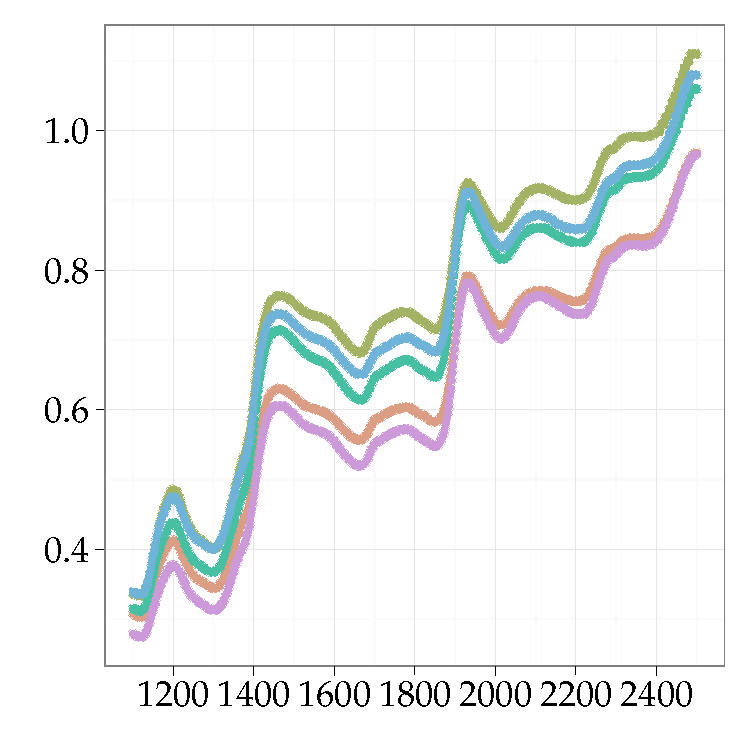
\includegraphics[width=\linewidth,height=\linewidth]{figure/graphics-GR_NIRspektrum} 

}


\end{knitrout}

  \end{minipage}
  \hspace{0.1cm}
  \begin{minipage}[c][][t]{0.48\textwidth}
    Eigenschaften der Daten?
    \begin{itemize}
      \item<1-> Hohe Anzahl an Beobachtungen im Vgl. zur Stichprobengr\"o{\ss}e
      \item<2-> \"Ahnlichkeit des Kurvenverlaufs, Daten sind collinear.
      \item<3-> Glatte Daten, aber komplexer zugrundeliegender Prozess
    \end{itemize}
    \hfill
  \end{minipage}
\end{frame}

%%%
%
%
%%%

\begin{frame}[fragile]
  \frametitle{Was sind funktionale Daten?}
  Im Allgemeinen geht man davon aus, dass 
  $$
    y_{ij} = x_i(t_{ij}) + \varepsilon_{ij},
  $$
  dabei sind die $t_{ij}$ diskrete Abtastungen einer kontinuierlichen Variable $t$
  (Zeit, Frequenz, usw.) und $x_i(t)$ die funktionalen Daten.\\
  \pause Daten erh\"alt man z.B. aus:
  \begin{itemize}
    \item Spektralen Messungen (z.B. Nahrungsmittelindustrie, Astronomie),
    \item Elektrischen Messungen (z.B. EKG, EEG),
    \item Audio-Messungen (z.B. Lungenger\"ausche, Sprache).
  \end{itemize}
  \pause Interpretation des Rauschens $\varepsilon_{ij}$ h\"angt von der Art der 
  Daten ab.
\end{frame}

%%%
%
%
%%%

\begin{frame}[fragile]
  \frametitle{Ausblick: Gl\"attung}
  \hspace{-0.1cm} 


  \begin{minipage}{0.48\textwidth}
  Niederschlag in Vancouver
\begin{knitrout}
\definecolor{shadecolor}{rgb}{0.969, 0.969, 0.969}\color{fgcolor}

{\centering 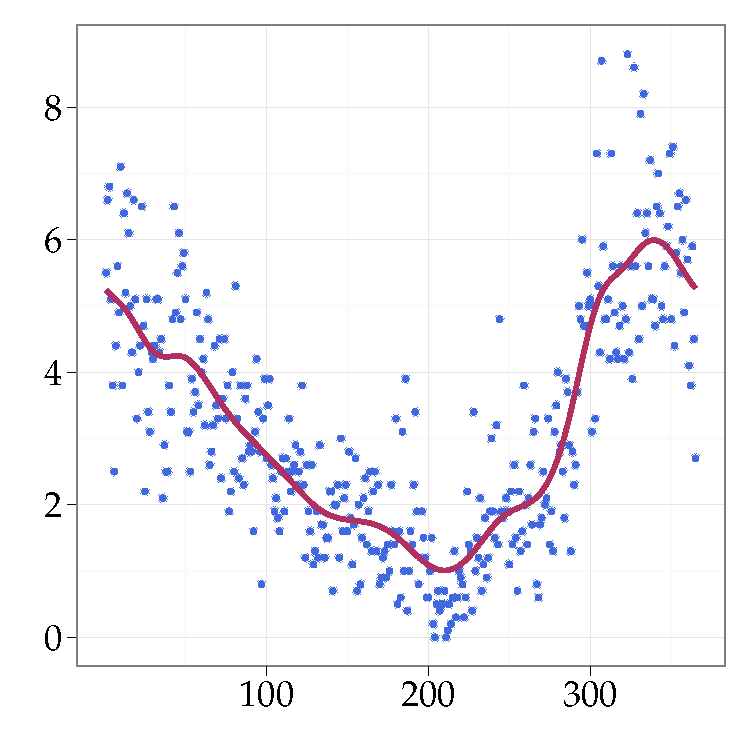
\includegraphics[width=\linewidth,height=\linewidth]{figure/graphics-GR_canada} 

}


\end{knitrout}

  \end{minipage}
  \hspace{0.1cm}
  \begin{minipage}{0.48\textwidth}
  log-Periodogramm zum Laut \textit{aa}
\begin{knitrout}
\definecolor{shadecolor}{rgb}{0.969, 0.969, 0.969}\color{fgcolor}

{\centering 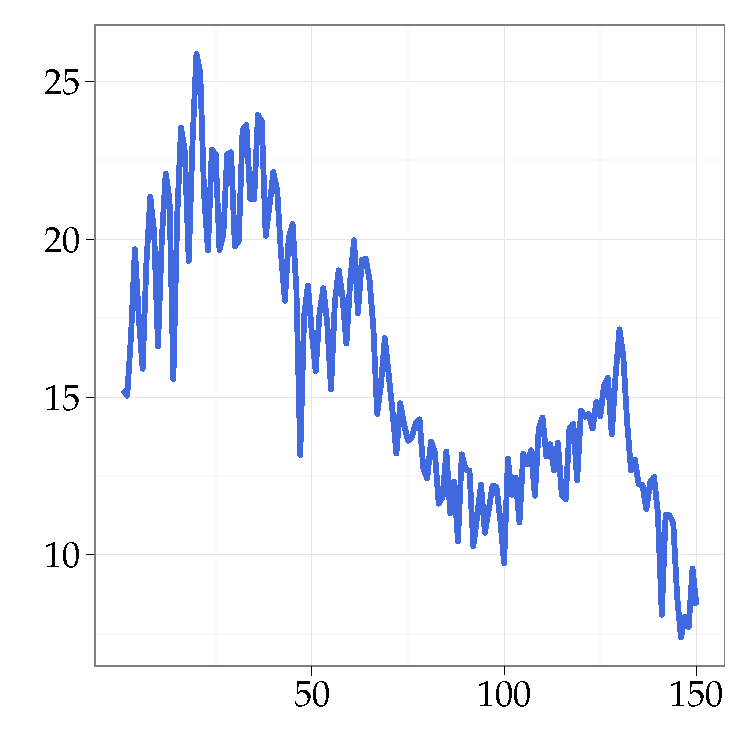
\includegraphics[width=\linewidth,height=\linewidth]{figure/graphics-GR_speech} 

}


\end{knitrout}

  \end{minipage}
\end{frame}

%%%
%
%
%
%%%

\subsection{Woran sind wir interessiert?}
\begin{frame}[fragile]
  \frametitle{Woran sind wir interessiert?}
  \begin{itemize}
    \item<1-> Deskriptive Darstellung von Funktionen
    \begin{itemize}
      \item<1-> Erwartungswert, Median
      \item<1-> Varianz
      \item<1-> Covarianz
    \end{itemize}
    \item<2-> Beziehung funktionaler Daten zu
    \begin{itemize}
      \item<2-> Antwortvariablen (z.B. Fettgehalt, Wort)
      \item<2-> Antwortfunktionen (z.B. Niederschlag pro Tag)
      \item<2-> den anderen Beobachtungen (z.B. Sterblichkeitsraten)
    \end{itemize}
    \item<3-> Beziehung zu den Ableitungen der funktionalen Daten (z.B. Dynamik 
              des Schreibens)
    \item<4-> Zeitereignisse in den Funktionen (z.B. Registrierung 
              Handschriftdaten)
  \end{itemize}
\end{frame}

%%%
%
%
%%%

\subsection{Worin liegen die Herausforderungen?}
\begin{frame}[fragile]
  \frametitle{Worin liegen die Herausforderungen?}
  \begin{itemize}
    \item<1-> Sch\"atzung der funktionalen Daten $x_i(t)$ anhand diskreter und 
              verrauschter Daten
    \item<2-> Numerische Repr\"asentation unendlich-dimensionaler Objekte
    \item<3-> Beschreibung statistischer Zusammenh\"ange zwischen unendlich-
              dimensionalen Objekten
    \item<4-> Darstellung der Variation in unendlich-dimensionalen R\"aumen
%    \item<5-> Kleine Stichprobe $n$, hohe Dimension $p=\infty$ (Fluch der   
%              Dimensionen)\\
%    Sei $\lambda$ das Lebesgue-Ma{\ss} auf $(I=[0,1]^p, \mathcal{B}(I))$, dann 
%  	$$\lambda(I) = 1 \textnormal{ und }\lambda(K) = \frac{1}{2^{p}} \dfrac{\pi^{p/2}}{\Gamma(p/2)}$$
  \end{itemize}
\end{frame}

%%%
%
%
%%%

\subsection{Referenzen}
\begin{frame}[fragile]
\frametitle{Referenzen (alle von Springer)}
  Parametrische funktionale Datenanalyse:  
  \begin{itemize}
    \item Ramsay, Hooker, and Graves, \textit{Functional Data Analysis
          with R and MATLAB}, 2009
    \item Ramsay and Silverman, \textit{Functional Data Analysis}, 2005
    \item Ramsay and Silverman, \textit{Applied Functional Data Analysis}, 
          2002
  \end{itemize}
  \pause Nichtparametrische funktionale Datenanalyse:
  \begin{itemize}
    \item Ferraty and Vieu, \textit{Nonparametric Functional Data Analysis}, 
          2007
  \end{itemize}
\end{frame}


%%%%%%%%%%%%%%%%%%%%%%%%%%%%%%%%%%%%%%%%%%%%%%%%%%%%%%%%%%%%%%%%%%%%%%%%%%%%%%%%
%
% Funktionale Varianzanalyse
%
%%%%%%%%%%%%%%%%%%%%%%%%%%%%%%%%%%%%%%%%%%%%%%%%%%%%%%%%%%%%%%%%%%%%%%%%%%%%%%%%

\section{Funktionale Varianzanalyse}
\begin{frame}[fragile]
  \frametitle{Gliederung}\tableofcontents[currentsection, subsection]
\end{frame}

%%%
%
%
%%%

\subsection{Datensatz: Vogelpopulation}
\begin{frame}[fragile]
\frametitle{Datensatz: Vogelpopulation}
% Hole Karte


  \begin{minipage}{0.48\textwidth}
    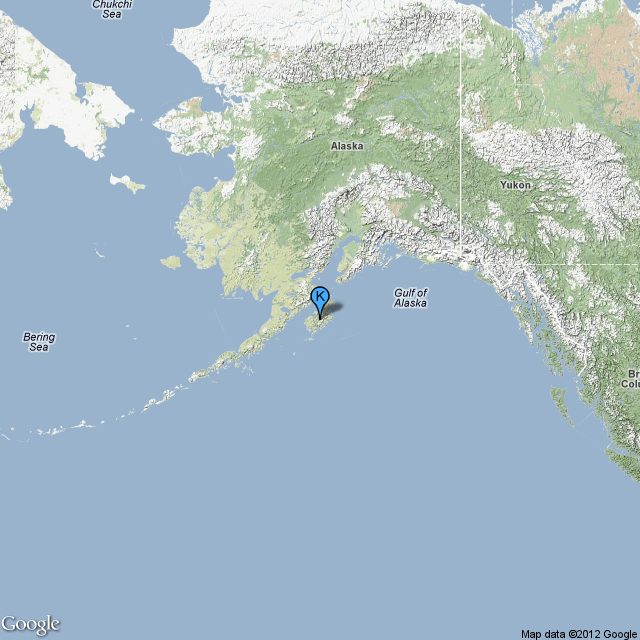
\includegraphics[width = 1.\linewidth, height = 1.\linewidth]{kodiak_insel.png}
  \end{minipage} 
  \hspace{0.1cm}
  \begin{minipage}{0.48\textwidth}
    \begin{itemize}
      \item<1-> Die Anzahl von $15$ Vogelarten wurde j\"ahrlich seit $1986$ im 
                Winter in einer Reihe von Buchten und festen Gebieten auf den 
                Kodiak Inseln (Alaska) von der \textit{Kodiak National Wildlife 
                Refuge} gez\"ahlt.
      \item<2-> In der nachfolgenden Analyse sind die Daten
                \begin{itemize}
                  \item auf die $2$ Buchten Uganik und Uyak beschr\"ankt und
                  \item es werden $13$ von den $15$ Vogelarten betrachtet.
                \end{itemize}
    \end{itemize}
  \end{minipage}
\end{frame} 

%%%
%
%
%%%

\begin{frame}[fragile]
\frametitle{Fragestellung}
  Es soll untersucht werden, ob und welchen Einfluss die Ern\"ahrung
  auf die Population der Vogelarten hat.
% Führe Vorberechnungen für die Grafiken aus


  \hspace{-0.1cm}   
  \begin{minipage}{0.48\textwidth}
\begin{knitrout}
\definecolor{shadecolor}{rgb}{0.969, 0.969, 0.969}\color{fgcolor}

{\centering 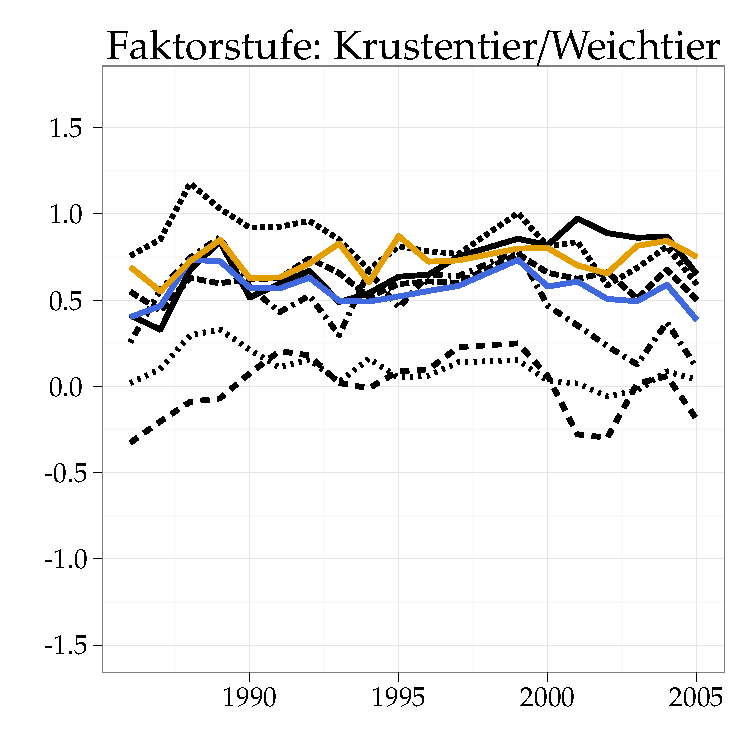
\includegraphics[width=\linewidth,height=\linewidth]{figure/graphics-GR_Krustentier} 

}


\end{knitrout}

  \end{minipage}
  \hspace{0.1cm}
  \begin{minipage}{0.48\textwidth} 
\begin{knitrout}
\definecolor{shadecolor}{rgb}{0.969, 0.969, 0.969}\color{fgcolor}

{\centering 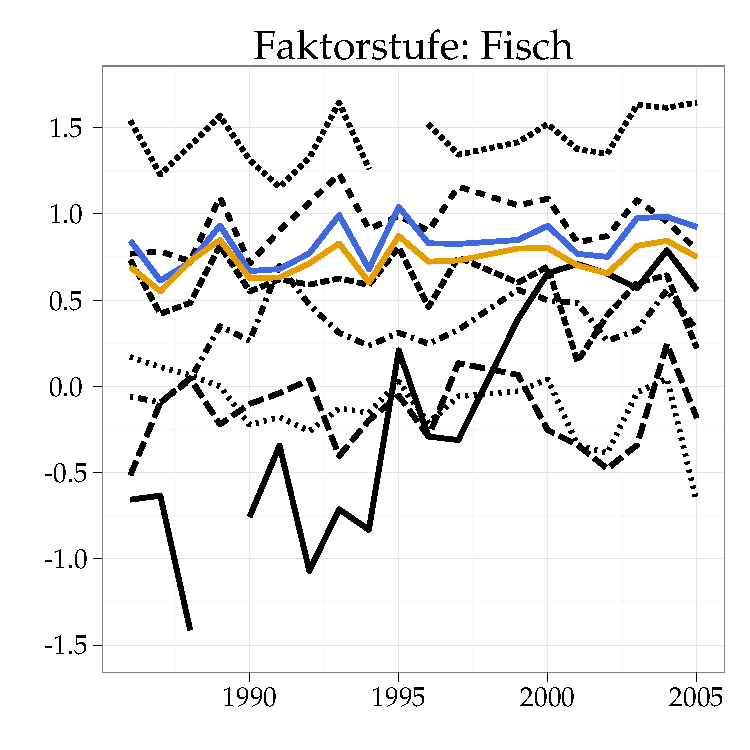
\includegraphics[width=\linewidth,height=\linewidth]{figure/graphics-GR_Fisch} 

}


\end{knitrout}

  \end{minipage}
\end{frame}

%%%
%
%
%%%

\begin{frame}[fragile]
\frametitle{Beschreibung}
  \begin{itemize}
    \item<1-> Es wird der Einfluss der Ern\"ahrung auf den zeitlichen 
          Trend der logarithmierten gemittelten Anzahl von V\"ogeln analysiert. 
    %\item<2-> Gez\"ahlt wurde in festgelegten Gebieten in jeder Bucht.
    \item<2-> Die Vogelarten werden in $2$ Faktorstufen ($=$ 
          \{\textit{Krusten- bzw. Weichtiere}; \textit{Fische}\}) eingeteilt
    \begin{itemize}
          \item<2-> Die Stichprobe zur FS \textit{Krustentiere} enth\"alt $n_1 = 6$ 
                Elemente
          \item<2-> Die Stichprobe zur FS \textit{Fische} enth\"alt $n_2 = 7$ Elemente
    \end{itemize}
    \item<3-> Zeitraum: $1986-2005$ (ohne $1998$) 
  \end{itemize}
\end{frame}

%%%
%
%
%%%
\subsection{Das Modell}
\begin{frame}[fragile]
\frametitle{Das Modell}
Wir betrachten folgendes Modell:
$$
y_{ijk}(t) = \mu(t) + (-1)^{i} \alpha(t) + \beta_{ij}(t) + \varepsilon_{ijk}(t)
$$
\begin{itemize} 
  \item<1-> $i=1,2$ indiziert die Nahrungsquelle
  \item<2-> $j = 1,\ldots,n_i$ indiziert die Vogelart in der jeweiligen 
        Nahrungsgruppe
  \item<3-> $k = 1,2$ indiziert die Bucht
  \item<4-> Der funktionale Parameter $\mu(t)$ bezeichnet den mittleren globalen 
        Trend \"uber alle Vogelarten.
\end{itemize}
\end{frame}

%%%
%
%
%%%

\begin{frame}[fragile]
\frametitle{Das Modell}
Wir betrachten folgendes Modell:
$$
y_{ijk}(t) = \mu(t) + (-1)^{i} \alpha(t) + \beta_{ij}(t) + \varepsilon_{ijk}(t)
$$
\begin{itemize}  
  \item<1-> Der Parameter $\alpha(t)$ bezeichnet den Trend \"uber die mittlere
        Differenz zwischen den Krusten- bzw. Weichtier und den Fisch 
        essenden Vogelarten.
  \item<2-> $\alpha(t)$ wird mit $1$ multipliziert, wenn die Beobachtung zu einer Krusten- 
        bzw. Weichtier essenden Vogelart geh\"ort und mit $-1$ bei einer Fisch 
        essenden.
  \item<3-> Der Parameter $\beta_{ij}(t)$ bezeichnet den Trend, welcher die 
            Abweichungen von $\mu(t)$ darstellt, f\"ur jede Vogelart, die zu einer der 
            Nahrungsgruppen geh\"ort.
\end{itemize}
\end{frame}

%%%
%
%
%%%

\begin{frame}[fragile]
\frametitle{Das Modell}
$$
y_{ijk}(t) = \mu(t) + (-1)^{i} \alpha(t) + \beta_{ij}(t) + \varepsilon_{ijk}(t)
$$
\begin{itemize}  
  \item<1-> Dies wird f\"ur alle $t$ erreicht durch die Nebenbedingungen
        $$
          \sum\limits_{j=1}^{n_1}\beta_{1j}(t) = 0 \textnormal{ und } 
          \sum\limits_{j=1}^{n_2}\beta_{2j}(t) = 0.
        $$
  \item<2-> Der Parameter $\varepsilon_{ijk}(t)$ bezeichnet die Residuen.
  \item<3-> Kein Einfluss: Bucht und der Interaktion von Bucht $*$ Nahrung
  \item<4-> Dies ergibt $28$ Gleichungen: $2$ Bl\"ocke der $13$ Vogelarten und die 
        beiden Nebenbedingungen. 
\end{itemize}
\end{frame}

%%%
%
%
%%%

\subsection{Resultat}
\begin{frame}[fragile]
\frametitle{Resultat}
% Führe fANOVA durch


  \hspace{-0.1cm}   
  \begin{minipage}{0.48\textwidth}
      Zeitlicher Trend $\mu(t)$ \"uber alle Vogelarten und Nahrungsquellen
\begin{knitrout}
\definecolor{shadecolor}{rgb}{0.969, 0.969, 0.969}\color{fgcolor}

{\centering 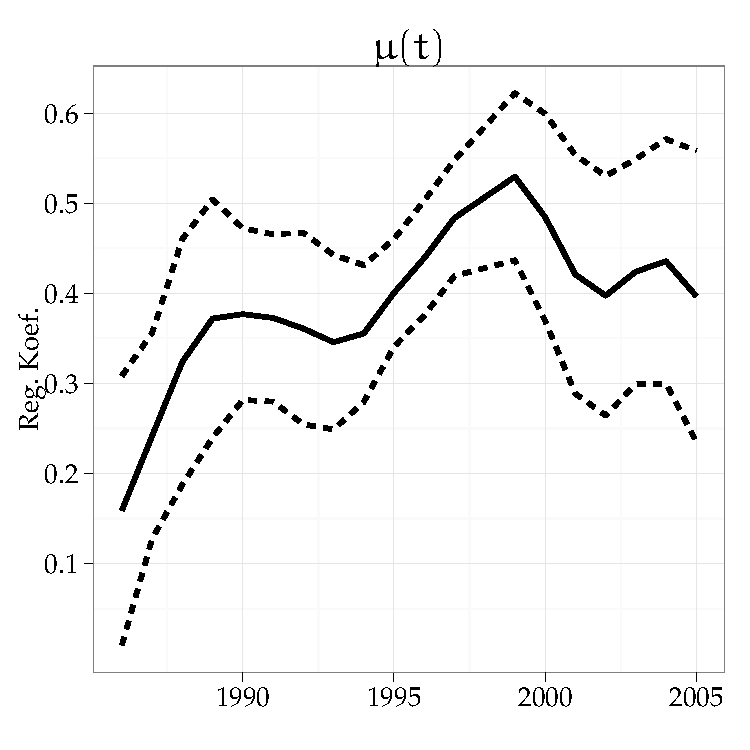
\includegraphics[width=\linewidth,height=\linewidth]{figure/graphics-GR_ANOVA_mu} 

}


\end{knitrout}

  \end{minipage} 
  \hspace{0.1cm}
  \begin{minipage}{0.48\textwidth}
  Zeitlicher Trend $\alpha(t)$ \"uber die mittlere Differenz 
\begin{knitrout}
\definecolor{shadecolor}{rgb}{0.969, 0.969, 0.969}\color{fgcolor}

{\centering 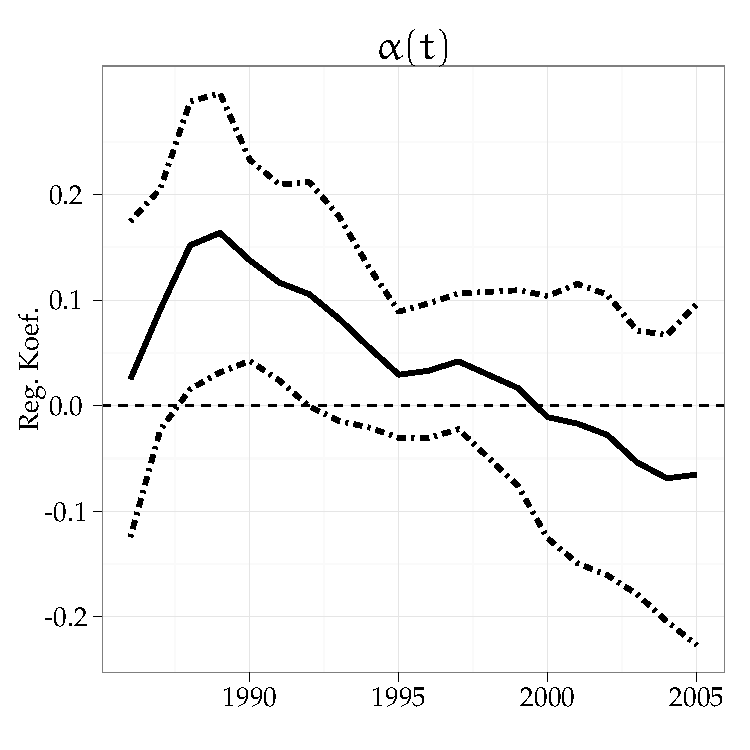
\includegraphics[width=\linewidth,height=\linewidth]{figure/graphics-GR_ANOVA_alpha} 

}


\end{knitrout}

  \end{minipage}
\end{frame}

%%%%%%%%%%%%%%%%%%%%%%%%%%%%%%%%%%%%%%%%%%%%%%%%%%%%%%%%%%%%%%%%%%%%%%%%%%%%%%%%
%
% Linear Funktionales Modell mit Funktionaler Beobachtung
%
%%%%%%%%%%%%%%%%%%%%%%%%%%%%%%%%%%%%%%%%%%%%%%%%%%%%%%%%%%%%%%%%%%%%%%%%%%%%%%%%

\section{Lineares Funktionales Modell mit Funktionaler Beobachtung}
\begin{frame}[fragile]
  \frametitle{Gliederung}\tableofcontents[currentsection, subsection]
\end{frame}

%%%
% 
%
%%%

\subsection{Datensatz: Sterblichkeitsraten schwedischer Frauen}
\begin{frame}[fragile]
\frametitle{Datensatz: Sterblichkeitsraten schwedischer Frauen}


  \hspace{-0.1cm}   
  \begin{minipage}{0.48\textwidth}
\begin{knitrout}
\definecolor{shadecolor}{rgb}{0.969, 0.969, 0.969}\color{fgcolor}

{\centering 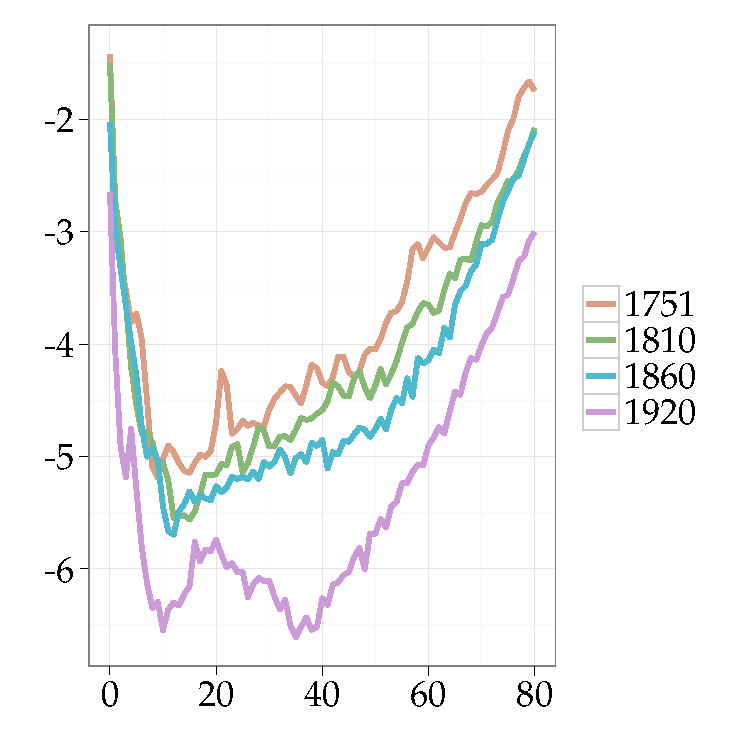
\includegraphics[width=\linewidth,height=\linewidth]{figure/graphics-GR_bspmort} 

}


\end{knitrout}

  \end{minipage} 
  \hspace{0.1cm}
  \begin{minipage}{0.48\textwidth}
    \begin{itemize}
      \item<1-> Logarithmierte Hazardrate schwedischer Frauen im Alter von $0$ bis
            $80$ Jahren.
      \item<2-> Berechnet aus Daten von: \url{www.mortality.org} 
      \item<3-> Zeitraum Datensatz: $1757$ -- $1900$
    \end{itemize}
  \end{minipage}
\end{frame}

%%%
%
%
%%%

\begin{frame}[fragile]
\frametitle{Datensatz: Sterblichkeitsraten schwedischer Frauen}


  \hspace{-0.1cm}   
  \begin{minipage}{0.48\textwidth}
\begin{knitrout}
\definecolor{shadecolor}{rgb}{0.969, 0.969, 0.969}\color{fgcolor}

{\centering 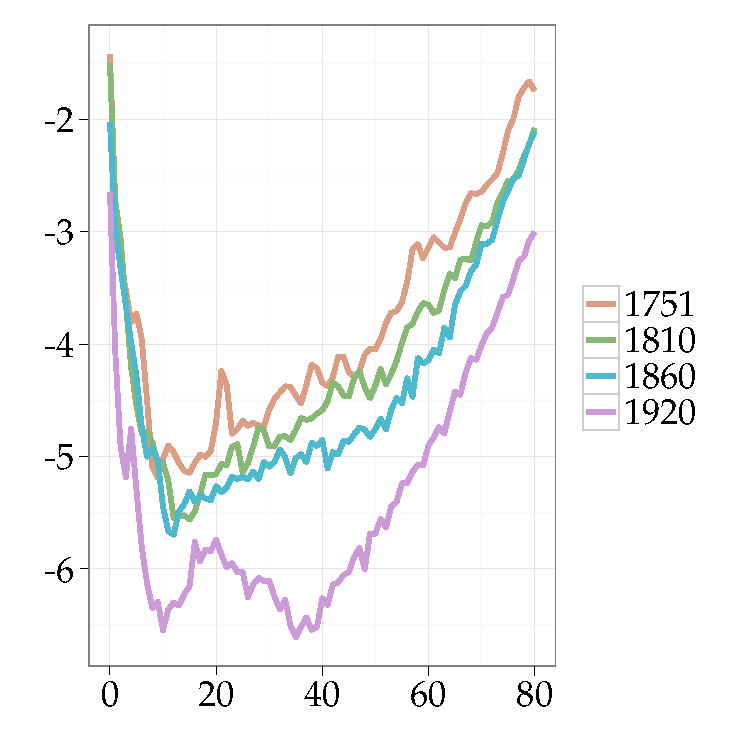
\includegraphics[width=\linewidth,height=\linewidth]{figure/graphics-GR_bspmort} 

}


\end{knitrout}

  \end{minipage} 
  \hspace{0.1cm}
  \begin{minipage}{0.48\textwidth}
    Sterbewahrscheinlichkeit ist
    \begin{itemize}
      \item<1-> im S\"auglingsalter besonders hoch,
      \item<2-> hat ein Minimum im Teenageralter
      \item<3-> und nimmt mit dem Alter zu.
      \item<4-> Mit zunehmender Gesundheit nimmt die Sterbewahrscheinlichkeit ab.
      \item<5-> Lokale Ausschl\"age entsprechen z.B. Kriegen, Krankheiten, usw.
    \end{itemize}
  \end{minipage}
\end{frame}

\begin{frame}[fragile]
\frametitle{Datensatz: Sterblichkeitsraten schwedischer Frauen}


  \hspace{-0.1cm}   
  \begin{minipage}{0.48\textwidth}
\begin{knitrout}
\definecolor{shadecolor}{rgb}{0.969, 0.969, 0.969}\color{fgcolor}

{\centering 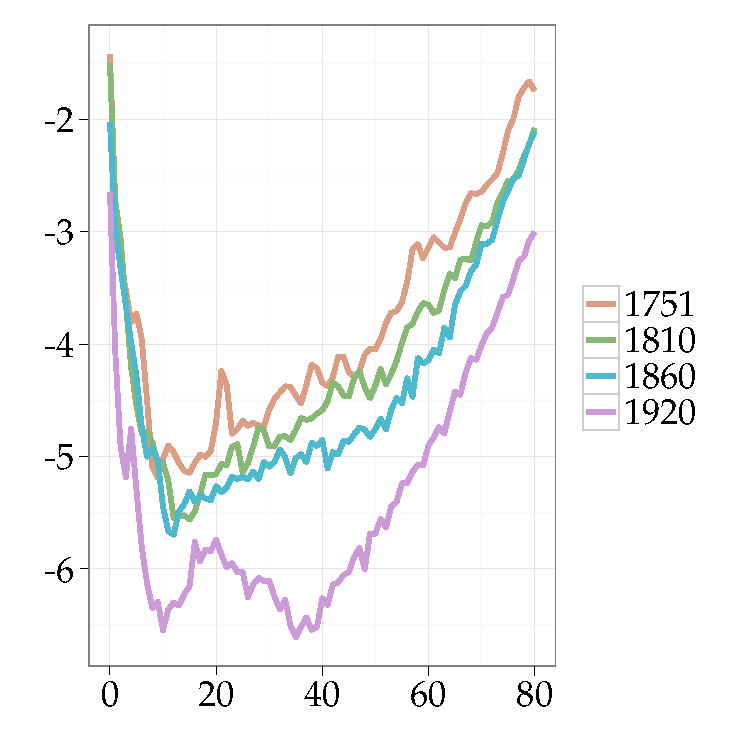
\includegraphics[width=\linewidth,height=\linewidth]{figure/graphics-GR_bspmort} 

}


\end{knitrout}

  \end{minipage} 
  \hspace{0.1cm}
  \begin{minipage}{0.48\textwidth}
\begin{knitrout}
\definecolor{shadecolor}{rgb}{0.969, 0.969, 0.969}\color{fgcolor}

{\centering 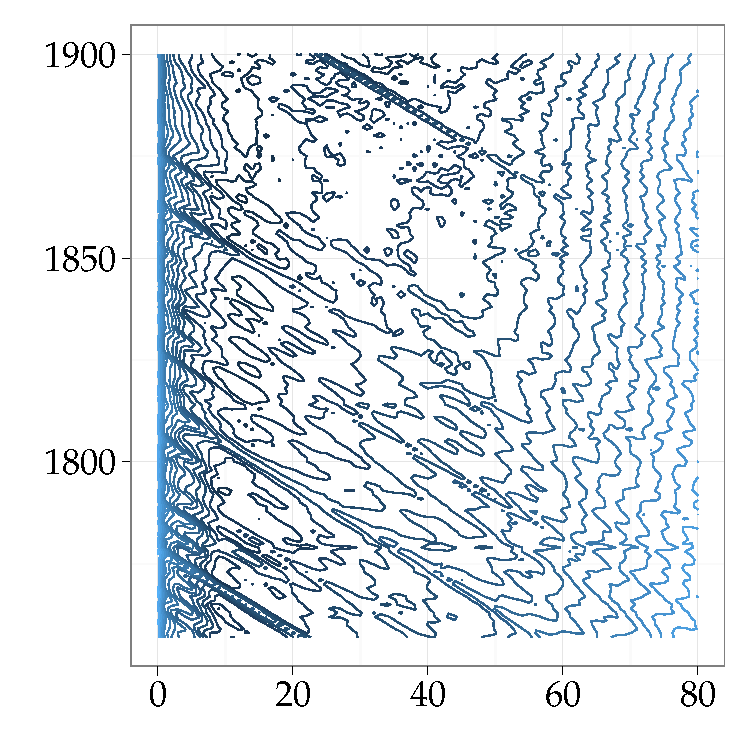
\includegraphics[width=\linewidth,height=\linewidth]{figure/graphics-GR_res_org} 

}


\end{knitrout}

  \end{minipage}
\end{frame}

%%%
%
%
%%%

\subsection{Das Modell}
\begin{frame}[fragile]
\frametitle{Das Modell}
  Wir passen folgendes Auto-regressives Modell an die Daten an: 
  $$
    x_{i+1}(t) = \beta_0(t) + \int_{\Omega_t} x_i(s) \beta_1(s, t)ds + \varepsilon_i(t)
  $$
  \begin{itemize}
    \item<1-> $x_i(t)$ logarithmierte Hazardrate f\"ur die Jahre 
          $i = 1757, \ldots, 1900$ zum Alter $t\in [0, 80]$
    \item<2-> Integrationsgebiet $\Omega_t = [0, 80]$
    \item<3-> $\varepsilon_i(t)$ Rauschen
  \end{itemize}
\end{frame}

%%%
%
%
%%%

\subsection{Resultat}
\begin{frame}[fragile]
\frametitle{Resultat}
  \begin{minipage}{0.48\textwidth}
\begin{knitrout}
\definecolor{shadecolor}{rgb}{0.969, 0.969, 0.969}\color{fgcolor}

{\centering 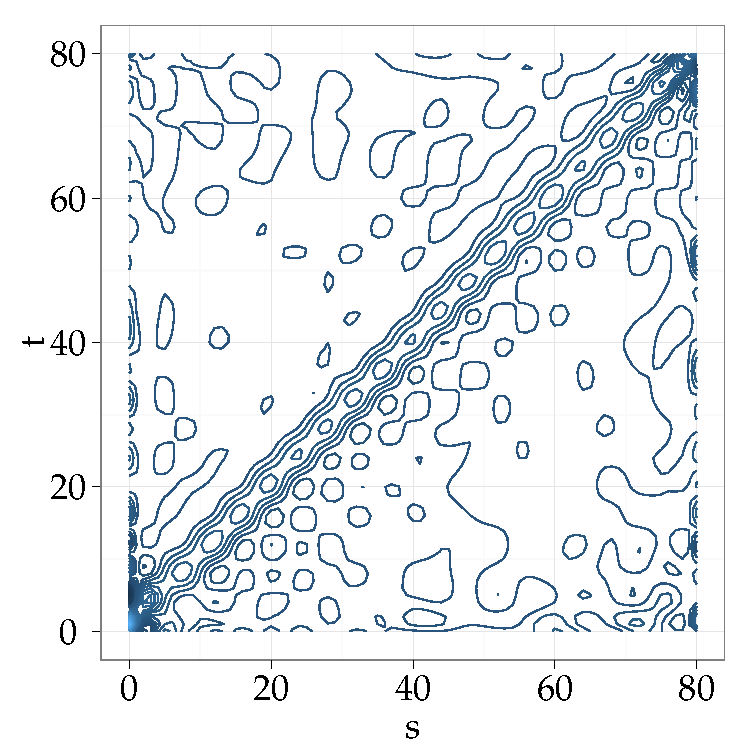
\includegraphics[width=\linewidth,height=\linewidth]{figure/graphics-GR_res} 

}


\end{knitrout}

  \end{minipage} 
  \hspace{0.1cm}
  \begin{minipage}{0.48\textwidth}
    \begin{itemize}
    \item $\beta_{0}(t) \approx 0$
    \item $x_{i+1}(t) \approx \int x_i(s) \beta_1(s, t)ds$ 
    \item Die Koeffizienten haben einen Einfluss auf der Diagonalen,
    $\beta_1(s-1, s)$
    \item Sterblichkeitsrate des aktuellen Jahres steht in Beziehung zu der 
    im vorigen Jahr
 \end{itemize}
  \end{minipage}
\end{frame}
 
  
%  Originaldaten
%<<GR_res_org, echo=FALSE, out.height='\\linewidth', out.width='\\linewidth'>>=
%@
%%%
%
%
%%%

\section{Eigene Forschung}
\begin{frame}[fragile]
\frametitle{Eigene bisherige Forschung}
  \begin{itemize}
    \item<1-> Nichtparametrische Regression:
    $
      Y = m(X) + \varepsilon
    $
    \begin{itemize}
      \item<1-> f\"ur funktionale und 
      \item<1-> $\alpha$-mischende Daten.
      \item<1-> Sch\"atzer: Nadaray-Watson Kernsch\"atzer
    \end{itemize}
    \item<2-> Bandweitenwahl
    \begin{itemize}
      \item<2-> k-N\"achste Nachbarn Kernsch\"atzer
      \item<2-> Bootstrapping
    \end{itemize}
    \item<3-> Gleichm\"a{\ss}ige Konvergenzaussagen
  \end{itemize}
\end{frame}

%%%
%
%
%%%

\section{}
\begin{frame}[fragile]
  \begin{center}
		\Huge{\textbf{Vielen Dank f\"ur Ihre Aufmerksamkeit!}}
	\end{center}
\end{frame}

\end{document}
